\chapter*{外\quad 文\quad 译\quad 文}
\pagestyle{empty}

\begin{center}
{\heiti\zihao{3}HotDrink}

{\heiti\zihao{4}A Library for Web User Interfaces}

\textsl{By John Freeman, Jaakko Järvi, Gabriel Foust}

{\heiti\zihao{3} HotDrink}
\end{center}

\zihao{-4}

\section*{摘要}
HotDrink是一个用于创建表格、对话框以及其他Web应用常用的用户界面组件的JavaScipt库。使用HotDrink,开发者用JavaScript声明了一个“视图模型”,并在模型与组成视图的HTML 元素之间建立一系列的“绑定”。这些规范虽然微不足道,但足够让HotDrink提供一个全功能的GUI,包括多路数据流、启用/禁用数值、激活/无效命令以及数据验证。HotDrink以高质量的用户接口将这些丰富多彩的行为实现为可重用代码。这篇文章以及工具演示通过逐步的展示一个Web应用GUI的构建过程,向开发者介绍HotDrink库。
\section*{前言}
用户界面(UI)编程往往费时费力。有研究表明,创建应用时,UI实现的代码平均占40\%[14],另一个研究为平均30\%[10]. 这些数字很高但可能并不令人惊讶;UI实现往往需要大量的、不可重用的、此应用专属代码。
一个典型的图形UI库提供的主要服务就是将用户行为转化为事件并将事件递交给相应的事件处理函数。UI程序员写出事件处理程序并注册去监听相应事件。这也是目前主要的Web UI编程模型;UI行为在事件处理程序中用程序逻辑定义好。
随着编程社区逐渐接受事件处理程序模型,其他方法已经且正在被寻找。我们定义了两个趋势:(1)用宣告式数据流约束代替命令式事件处理;(2)设计能帮助程序员分离数据展示和逻辑的模式
对第一个趋势,针对UI的数据流约束系统在过去几十年里被积极的研究过[5,13,16],并已经被使用,比如在UI元素的布局与排列中。最近的一些Web编程框架[2,1,3]也使用了约束来管理显示在UI控件中的变量,特别与观察者模式一起[8,5]。
至于第二个趋势,流行的设计模式的发展,从Model View Presenter[15],到Presentation Model[6],到Model View View Model[9],(MVVM), 反应了针对代码分离更好的设计的追求。这些模式中最新的,MVVM,其目标是创建没有逻辑,只需保留从用户行为保留事件、与从视图模型展示数据的任务。视图模型维护UI的状态,也就是与展示在控件上的内容密切相关的、能反应一部分模型数据的数据。模型是应用“业务”数据与逻辑的统一体,和在传统的MVC模式中一样[12]。
为实现宣告式的用户界面编程,HotDrink 采用我们的属性模型方法[10,11,7]。它结合了上述两种趋势:HotDrink中的视图不包含编程逻辑(通常他们只是HTML控件的声明),并且所有的UI状态被包含在一个视图模型中,这个模型被实现为多路数据流约束系统。HotDrink的最终代码简明清晰,因其对编程者隐藏了所有事件处理代码,并且将许多复杂的UI行为(变量传播、控件可用/禁用、命令激活/失活等等)实现为可重用算法
这篇文章/工具演示对HostDrink的主要功能进行了描述。我们将带着读者了解一个Web UI例子的实现的流程,来解释程序员视角——程序员创建一个GUI的时候要写的一系列说明。
最后,HotDrink的设计允许增量采用,如果需要,一部分用户界面可以受HotDrink控制,但另一部直接被JavaScript事件处理函数或其他的GUI框架控制。HotDrink在Object和Array原型上添加了一些方法,但不用担心这些附加会跟其他库冲突。
\section*{例讲程序员视图}
图1显示了典型酒店预订表单的一个部分。预订服务需要入住和离开时间以查询可入住的房间。增加“晚”这个字段之后,该UI提供了三种方法来指定这些日期――通过任意两个字段都能推断出第三个字段的值。我们将介绍如何使用HotDrink及Model-View-ViewModels模式来构造这个界面。读者可到hotdrinkjs.com/date-example下载实现代码。
\begin{figure}[!h]
  \begin{center}
    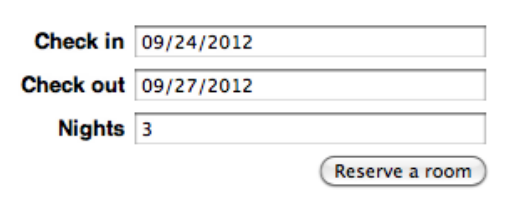
\includegraphics[scale=0.3]{figures/translation/translation_hotdrink_fig1.png}\\
    选择旅店住宿时段的表格
  \end{center}
\end{figure}
\subsection*{模型}
模型本身是在HotDrink范围之外。对于一个酒店预订应用,它的组成可能会包括一个房间、预订信息数据库以及普通查询的各种算法,比如检查是否有可用房间、增加或删除预订信息。HotDrink假定一个模型已经存在,然后帮助在这个模型之上构建一个用户接口。模型与视图之间的绑定应当由程序员实现,比如在一边移动数据以响应另一边的变化。HotDrink提供视图-模型的更改通知以支持这个任务。
\subsection*{视图-模型}
HotDrink API 提供一种嵌入式特定领域语言(在JavaScript中)来定义视图-模型。在这种语言中,程序员声明变量及它们之间的关系,一起组成这个视图-模型的约束Constraint系统。
所有API存在于hd命名空间。图2显示了酒店预订表单视图-模型的API规范。
\begin{figure}[!h]
  \begin{center}
    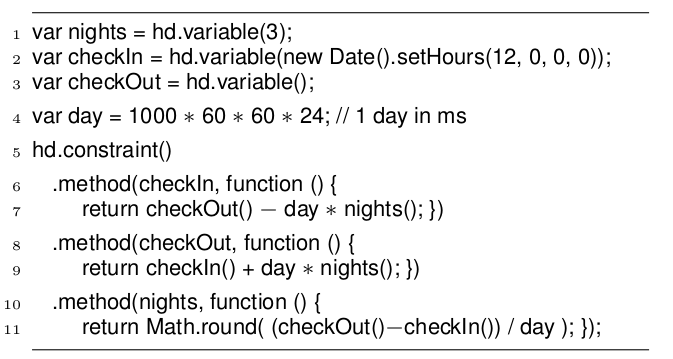
\includegraphics[scale=0.3]{figures/translation/translation_hotdrink_fig2.png}\\
    表格的视图模型
  \end{center}
\end{figure}
变量可赋予值。直接不加参数地使用这个变量可获得它的值,重新赋值时可将新值作为唯一的参数。图2所示的例子中有三个变量:分别为住几晚的数目、入住时间、离开时间。每个变量存储一个整数。两个日期变量以Unix epoch以来的毫秒表示。前两个变量以传递给hd.variable的值来初始化。在视图-模型的第一次更新(以下会介绍)时,最后一个变量由前两个变量得到初始化。
Constraints表达了变量之间的关系。每个Constraint由一组方法组成,每个方法是一个满足该Constraint(约束)的过程,――比如建立关系――使用其它变量作为输入,计算某些Constraint的变量的新值。在我们的例子里,唯一一个Constraint的声明开始于第5行,指定了三个方法。每个方法定义列出了它输出的一组变量,并以一个未命名的函数定义了这个方法的过程。
HotDrink要求程序员显式地指定一个Constraint的每个方法。对于某些关系,比如简单的相等,它有可能能够导出所有的方法,但这一点并不是对所有关系有效。将一个Constraint的变量划分成输入和输出组的每一次划分都定义了一个direction,并且,不是所有的direction都可能有关系, e.g., a one-way hash。
变量和Constraint一起组成了多向数据流Constraint系统。实现一个Constraint系统就是执行每个Constraint的一个方法,并且执行顺序不得使之前所满足的Constraint无效。在本文的其它地方我们对此进行了详细的介绍。
更新视图-模型(view-model) 实现了Constraint系统,并对于所有变量的变化发出了通知。增加一个变量或Constraint,写一个变量或显示的调用hd.update会引发一次更新。接受该通知的事件处理器将处理由view-model对model带来的响应,如上所述,并将处理由view-model对view带来的响应,如下所述。
HotDrink支持潜在Constraint系统的增量构造――可对已经与view绑定的系统增加新的变量和Constraint――这将允许view-model根据用户需求变化。
\subsection*{视图}
View和model一样,位于HotDrink的范围之外。View可由标准的HTML元素或者第三方widget工具包构造。我们的酒店预订表单的view是用Html写的,如图3所示。
\begin{figure}[!h]
  \begin{center}
    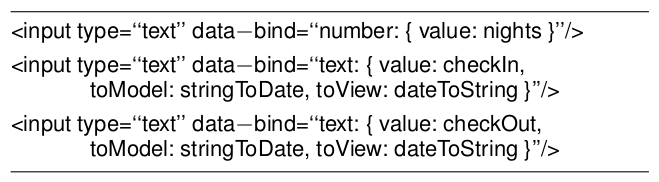
\includegraphics[scale=0.3]{figures/translation/translation_hotdrink_fig3.png}\\
    图1旅店预约表格的视图元素
  \end{center}
\end{figure}
Binding处理了widgets中view与view-model的变量之间的数据交换。它们可以是单向的(从view-model到view),或者是双向的。HotDrink为从views到view-models之间的binding提供了两种机制:javaScript或者Html属性。我们的例子选择了声明性binding,如图3所示。
Binder是一个函数,用来构造和注册一个事件处理器,后者实现某个特定的binding。比如,HotDrink文本binder将一个HTML文本输入widget与view-model的一个变量绑定,使用了两个事件处理器:
\begin{itemize}
  \item 第一个监听widget的变人,并写入变量
  \item 第二个监听变量的变化,并更新widget
\end{itemize}
事件处理器是如此的琐碎,因为view-model constraint 系统处理了UI数据之间的所有依赖。在view出现变化的情况下,第一个处理器为constraint系统的一个变量分配一个新的值,引发一次更新。在solve 了constraint系统之后,view-model通知第二个处理器它所负责的widget或许需要更新。
Binder包装了很多细节,包括观察view中的变化,更新view,以及将view中所使用的数据类型转换为view-model所使用的数据类型(反之亦然)。可以自定义binder来扩展hotdrink以支持任何view。在简单的情况下,binder只需要几句代码即可。HotDrink为标准的HTML widgets提供了内建binder。
构建binding时将一个widget和一组选项传递给一个binder。为了方便,binding可以在HTML中使用data-bind属性声明。这个属性是一个JSON对象,其键为binder名字,其值为binder选项。当指向成功,HotDrink用widges和配置数据调用各个已命名的binder。在构建复杂的binding时,比如为第三方使用javascript的jwidget构建binding时,程序员必须在javascript中显式地调用一个binder。
在酒店预订的例子中,见图3,每个binding使用上面提到的内建文本binder。Value选项命名了view-model中的相应变量。在很多情况下,比如这里的“晚”字段,没必要使用其它的选项。然而,数据字段要求更多的配置。它们在web表单中表现出越来越大的复杂度:在view中表示的数据与view-model中表示的数据并不一样。在本例子中,view中的日期为字符串,而view-model中为integer。因此binding使用toModel和toView两个选项来指明两种数据相互转换的函数:
\begin{verbatim}
function dateToString(m) {
  var d = new Date(m);
  return { value: (d.getMonth() + 1) + "/" +
  d.getDate() + "/" + d.getFullYear() };
}
function stringToDate(s) {
  var m = Date.parse(s);
  if (isNaN(m)) return { error: "Invalid date format" };
  else return { value: m };
}
\end{verbatim}
由于转换可能会失败,每个转换函数都会将转换结果标记为转换后的值或者错误。在我们的例子里,保证了从view-model到view的成功转换,因此不会返回错误。
如果一个转换函数出错,view-model的变量不会改变。因此,转换函数提供了“验证”服务,保证view-model不会更改为错误的值。
最后,程序员必须将view-model传递给HotDrink:
\begin{verbatim}
var viewModel = {
  nights: nights,
  checkIn: checkIn,
  checkOut: checkOut
}
hd.bind(viewModel);
\end{verbatim}

\subsection*{行为}
使用一个constraint系统来model一个用户界面各值之间关系的优点在于,可以将复杂的UI功能实现为可重用的算法。我们已经描述过一些这样的算法,包括当一个command的前提被违反时,使这个command widget失效。HotDrink实现了那个算法的升级版本。下面我们介绍如何使用它。
程序员首先声明一个command:一个持有延迟函数(deferred function)的变量,这个函数是用函数和其参数构造的(cf. Command pattern [8, x5]). 不论该command是否触发,deferred function将用这些参数调用。典型地,一个commmand将对model一些方法的调用打包,并将view-model的一些变量的值作为参数传递过去。对于酒店预订表单,一个预订房间的command举例如下:
(代码)
\begin{verbatim}
viewModel.reserve = hd.command(function () {
  return hd.fn(model.reserve)(checkIn(), checkOut());
})
\end{verbatim}
Hd.fn函数defer了model的reserve方法的调用 。该deferred 调用由一个匿名函数构建。这个函数形成了view-model中一个单向constraint的唯一方法。不管什么时候,只要这个deferred 调用的一个参数发生变化,这个command都会重新构建。通过分离构建和调用,hotdrink可以在一个command的执行之前确认它的依赖,并实现复杂的UI 行为,比如command activation和widget enablement.
一个widget,比如一个按钮,可以与一个command绑定,因此用户针对它的动作会触发这个command。HotDrink为这种情况提供了内建的command binder:
\begin{verbatim}
<button data−bind="command: reserve">
  Reserve a room</button>
\end{verbatim}
对于command的触发,程序员声明前提条件――boolean谓语――在command触发前必须满足。例如,预订command可能需要至少居住1晚:
\begin{verbatim}
hd.precondition(viewModel.reserve, function () {
  return nights() > 0;
})
\end{verbatim}
不管何时,如果前提条件未能满足,该command触发算法会发出一个事件,表明它应当失效。Command widget,比如以上所提到的按钮,能够监听到这个事件并让自己失效。内建的HotDrink command默认使用这种方式。
HotDrink可以扩展新的Behavior。尽管增加behavior需要大量的工作,但价值在于它们可以重用。
\section*{总结}
文中提到的UI例子很简单。其依赖可以用视图模型中一个单一的约束来表达。更大型的UIs可能有更复杂的依赖,甚至难以用专门的事件处理代码管理。HotDrink通过在约束系统中将依赖封装到约束,来帮助管理这种复杂性。程序员可以在封闭状态下推理出每个约束——HotDrink的约束系统管理着他们的聚集行为。
为演示HotDrink在一个略微复杂的UI中的使用,我们根据TodoMVC工程[4]的说明文档,实现了一个规范的“todo list”应用(http://hotdrinkjs.com/todomvc). TodoMVC应用在对比不同的JavaScript MVC框架时,是一个很好用的基准。HotDrink在简明方面很有竞争性。需要注意的是,TodoMVC不能帮助展示HotDrink的一些有别于其他框架的更强大的功能,比如多路或多输出约束,以及通用的可复用的UI行为。
HotDrink可在https://github.com/HotDrink找到,且还在开发中。我们向HotDrink扩充一些之前提到的可重用行为[7],比如撤销/重做功能,管理数据流方向的控制行为,以及数据流的可视化。
\section*{致谢}
这篇文章是建立在Grant No.0845061自然科学基金支持的工作的基础上的。



\newpage
\pagestyle{empty}

\begin{center}
{\heiti\zihao{3}Using Concept Maps to Evaluate the Usability of APIs}
\textsl{By Jens Gerken,Hans-Christian Jetter,Harald Reiterer }

{\heiti\zihao{3} 用概念图评估API可用性}
\end{center}

\zihao{-4}

\section*{摘要}
应用程序接口(API)是现存编码结构,如控件、框架、工具包等的接口。其对最终系统的质量有很大影响。因此确保开发者对接口的最优使用是一项重要挑战。然而现有的来自HCI的标准可用性评估方法在开发者与API交互的理解上有一定限制——GUI这种明显的基于交互的接口就不能被评估。这篇文章中,我们展示了一个纵向方法,此方法使用概念图和问题笔记使得交互可见,随之能够研究API的可用性。

\section*{前言}
现今开发一个软件系统往往不需要从头做起,开发者经常可以依赖现有的控件、框架、库或软件开发工具包,等能提供现成代码来重用的工具。为了达到这个效果,需要提供应用程序接口(APIs),虽然可能已经有好多不同的APIs面向同一种应用目的。就像Daughtry et al.[4]说的“他们分别对同一个模块提供了程序接口”。这些接口中,其中一些比另其他的可用性更强,因此最近几年,对APIs可用性的研究被越来越多的研究者重视[e.g 4.5].从这些研究中,我们定义了两个主要目标。一个是在更通用的角度上分析APIs的使用方法,从而能为创建新的APIs或修改现有APIs衍生出设计原则。第二个是评估某个特定API的可用性,尤其是开发过程中作为以用户为中心的迭代生命周期的一部分的API。这篇文章中,我们主要关注第二点,我们提出了一个纵向评估方法,用来评定开发者在使用API及其更新版本的时候遇到的阻碍。
\section*{评估API的挑战}
评估一组API与标准的可用性评估很不同,最不一样的是丢失GUI,因此使用并与API互动比用标准软件应用更为难以捉摸,也更难观察和分析。相应的,这不是单纯的定义错误做法或用户观察时的错误标准,因为达到目的的方法有很多。从方法论的角度,最常用的方法是实验室内部结合起来进行有声思维的可用性测试。举例来说,Klemmer et al.[10]呈现了这样一个可用性研究:7个参与者使用Papier-Mâché Toolkit来开发有形的用户接口。参与者首先被介绍工具包,然后被要求用这个工具完成三个典型的任务。有声思维与参与者的Java代码被用来分析这个工具包的可用性。Heer et al.[9]分析Prefuse工具包用了相似的方法。另一个有趣的方法是Beaton et al.[2]提出来的。参与者首先用伪代码写下对于一个特定任务,他们期望API能做什么,然后用API真正执行这个任务。这样就能很好的评测出用户头脑中的模型与现实中的对比。
这些研究使用定量测量标准往往是完成任务的次数[5,1],有时是代码行数[10],或者需要的迭代步骤[1]。虽然这些有助于比较不同的APIs[5],他们只能从广义上指出可用性问题。有声思维与录像观察的更多细节分析有助于识别更多潜在的可用性问题。然而找出一系列或成簇的可用性问题很困难。一个可能的方法是Clarke提出的[3]。他使用认知维度框架并使其匹配API可用性评估的需求。通过使用此框架,评测者可以将从不同范畴找到的问题聚集,并因此可以识别出那些更高层次的API概念可能是有问题的。另一方面,Ko et al.[11]在大量研究中识别了一组API中的6个学习阻碍,这个方法可以用来聚集定性数据。识别这样的学习障碍与评测一组API的阈值只有一步之遥,这意味着要获得一个想要的输出有多难,Myers将其定义在他们的阈值和上限质量标准。这个上限定义了一组API中什么是可实现的。针对这类事件,一般的评估API的方法是案例研究,这些研究展示了一系列可能的系统。因此关于此类API可用性研究的分析,还有相当多的工作要做。我们认为从方法论的角度,还有提升的空间。现有方法在解决两方面不够充分:1)因为大多数研究被限制在一个或几个小时来测试,任务都比较简单且大多数时间被“事先定义”。那种可以用API完成的更复杂或“不受约束”的任务,很少并且在这样的研究设计中难于集成,尽管这样的任务能提供针对实际使用API的可用性很有价值的输入。2)在这样有代表性的研究中,评测学习障碍或API阈值似乎很难。需要做出长时间使用过程中障碍转化或者阈值很难设定等假设。这两方面问题都可以通过纵向研究设计解决,此设计主要收集多于一个时间点上的数据,这使得整合更复杂的任务和观察变化成为可能。在之后的章节中,我们会展示概念图方法来解决这些问题。它基于纵向领域研究设计和API用法可视化。
\section*{概念图方法}
我们方法的基础是概念图:我们在例会中观察开发者组,在这个两人的组中,他们要画一个能表现他们建立的系统和API之间的关系的图(见图1)。为了完成这项任务,参与者被要求在便利贴上做标注,并将其放到一张大纸上(见图1)。这张概念图不仅能显现开发者使用了哪部分API,还能展示出他们对于如何将这些API合作起来的思考。我们规定两人一组,这样他们就能组内讨论概念图的设计,大声交谈,并给出在理解此API方面有价值的见解。这样的一个概念图图示使得跟踪变化更为简单。
\begin{figure}[!h]
  \begin{center}
    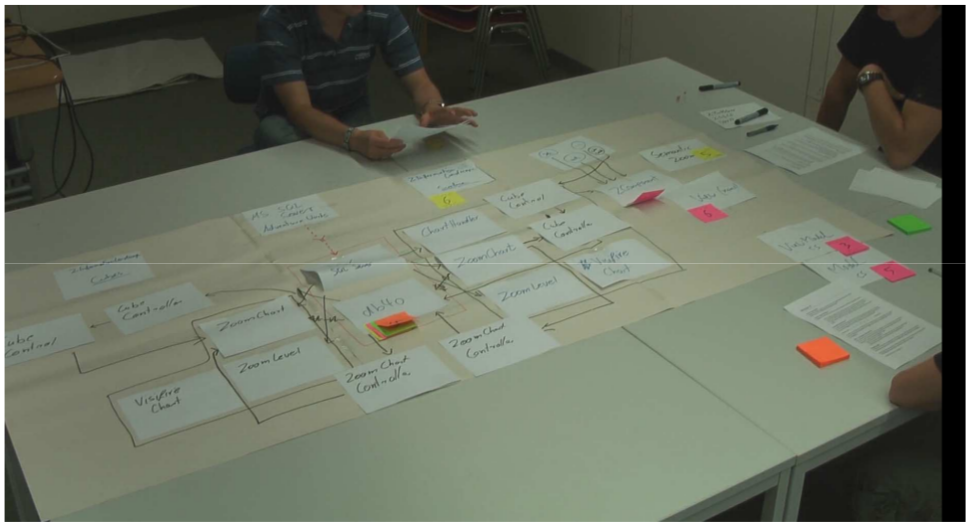
\includegraphics[scale=0.3]{figures/translation/translation_api_fig1.png}\\
    概念图实例
  \end{center}
\end{figure}

为了能理解实际的API使用时的体验,我们考虑使用基于远程数据集合技术的概念图。根据diary technique[13]和Grossman et al.[8]介绍的question-suggestion protocol, 我们使用questioning-diary方法。日记使我们能够从用户的日常工作环境中获得数据,而不是他们感到被监视时的数据。我们建议给参与者们这样一种感觉:以帮助栏的方式使用日记,即以问题的形式记录遇到的难题。概念图会议还应当包含建议/反馈环节,此环节中可以进行问题讨论,有可能的话请专家或API设计者来回答。这样的话,更深入地分析API成为可能,因为我们避免了从一开始参与者就被卡住的危险。日记实现可以通过多种方法,其中最简单的是用Wiki。这使得参与者不仅能声明问题还能在解决方法出现时随时更新,另外还令跟踪和分析变化成为可能。这两种方法都考虑到了进一步修改与调整。因此,我们目前已经展示应该被看做是这个方法的抽象展示。下一章节我们会以一个具体的此方法的“实现”为例,此外还会指出一些优点和现存缺陷。
\section*{ZOIL案例研究}
HCI领域的纵向研究的应用依然很少见,尽管需要这类研究的意识正在不断增强。为了给HCI领域的纵向研究建立一个普通的方法论基础,Gerken \& Relterer[7] 提出了一个体系,此体系主要展示了一个纵向研究的设计空间。在这个案例研究过程中,我们将参考这个体系进行构造。
\textit{ZOIL API}
Zoomable Object-Oriented Information Landscape (ZOIL) API, 是由本文其中一个作者开发的,提供访问ZOIL 框架服务的接口,部署在一个用C\#/XAML写给.NET和Windows Presentation Foundation (WPF)的软件框架上。它为程序员提供了一个具备各种不同功能的可扩展的类的集合,e.g.ZUIs,客户机-服务器持续性。它主要作为工具包,为开发以实际交互和表面计算为背景的可缩放用户接口服务。
\textit{研究目的、研究和数据收集设计}
我们首要的研究目的是定义使用API时的墙和障碍,以及他们之后可能会怎样变化。为了能获得一个足够大范围的API用法,我们选择多个案例研究设计,这与MILC方法相似[14].。 我们观察了两人一组共四个组,每组做不同的项目。目标是对每个案例,在以事实为基础的交互和表面计算的环境下,专为ZOIL框架,创建一个可运行的高保真的原型。所以数据和任务不是被研究者事先定义的,而是由参与者自行定义。这使得我们可以在现实条件下观察API的使用情况,而不存在在API可用性研究时预先定义任务和数据造成的偏差。我们的测试开发者是视觉信息搜寻系统报告的学生。我们用了5周的事件,在这期间每周三我们实施概念图例会,共进行了四次,每组分开进行。日记方法在基于事件的现场数据提取方面还可以有更大提高。
\textit{数据收集方法}
我们将给出更多与实现两个数据收集方法相关的细节。首先关于概念图方法,我们要求参与者们除了放置并连接概念外,还有将他们在1到7之间排序,1为“我一点也不喜欢这个概念”,7为“我真的很喜欢这个概念”。除此之外,他们需要用描述这个概念的形容词来表示排名,比如“整洁的”或者“不简明”。另外在会议期间,我们要求参与者精炼排名和他们给出的属性词,方便之后追踪过程。在最后一个会议上,我们给参与者们一些附加的API概念,让他们将其放入他们的概念图中,并解释他们会不会以及会怎样使用新的概念。这有利于我们进一步详细阐述他们对API和底层框架的理解。
\textit{数据分析}
日记和概念图两个方法的设计都允许我们能在定性数据的基础上分析变化。重点在让这些变化能清晰明确地呈现出来,比如通过让用户在每次会议过程中精简排名和形容词,精简概念图结构。这会导致强烈的但是简单的视觉上的改变,比如概念的转变、移除以及日记上已解决的被标记的问题。
\section*{初成果与展望}
本章节我们举例说明我们方法的潜力,并给出一些现有实现过程中观察到的缺陷。
以wiki为日记的方法在定期使用方面依然有困难。这导致一些不会在日记上报告的小问题,以及有时一些大点问题的状态不会在研究过程中被实时更新,这为判断数据可靠性增添了困难。我们建议用一个不太起眼的工具,把日记直接集成到IDE或工具包中。一个有趣的方法是使用twitter作为这个不起眼的工具以及低层次技术。除此之外,我们的参与者在找合适的词去描述API概念的时候遇到了问题。一个可能的解决方案是提前提供形容词,负面和正面词都应包括,然后让参与者从这些样本中挑选就行了。
概念图被证实在将用户对API的思维模型可视化这一方面很有用。在一些案例中,参与者将ZOIL底层框架更深层次的概念加入到自己的图中,并表示他们期望这些一直作为API的一部分。此外,在概念图创建过程中,组员之间的讨论对了解他们对API的理解和用法极为有帮助。概念图分析随着时间推移表现出惊人的洞察力。一个例子是由API提供的数据库连接,实际上不是用在数据存储,而是用来在多显示屏上系统同步的。有一组在这个问题的理解上出现了偏差,因此在他们的概念图中,即使有数据存储的需求,他们仅仅加入了db4o词API提供的后端连接。在第二周,他们意识到还不够,于是加入了MySQL数据库这个附加概念,并将其与db4o后端结合(见图2\&3)。识别学习障碍的一个例子是Model-View-ViewModel(MNNM)模式的用法(见图4)。正如所预料的, 其中有一组在集成上遇到了困难,在最后的时候才想出解决方案。然而,概念图表明(图5\&6)他们最终以一个近似基本的视图和模型分离方案告终。因此即使MVVM模式提供了所需要的功能,它也会被明显的归为一个API学习障碍。问题日记在概念图会议的讨论触点上还是有用的,帮助我们获得了对特定问题的更多见解。我们在最后一次会议集成进的附加任务,即要求参与者将API概念放入他们各自的图中,并给出在思考和理解API方面上的更多见解。

\begin{figure}
  \begin{center}
    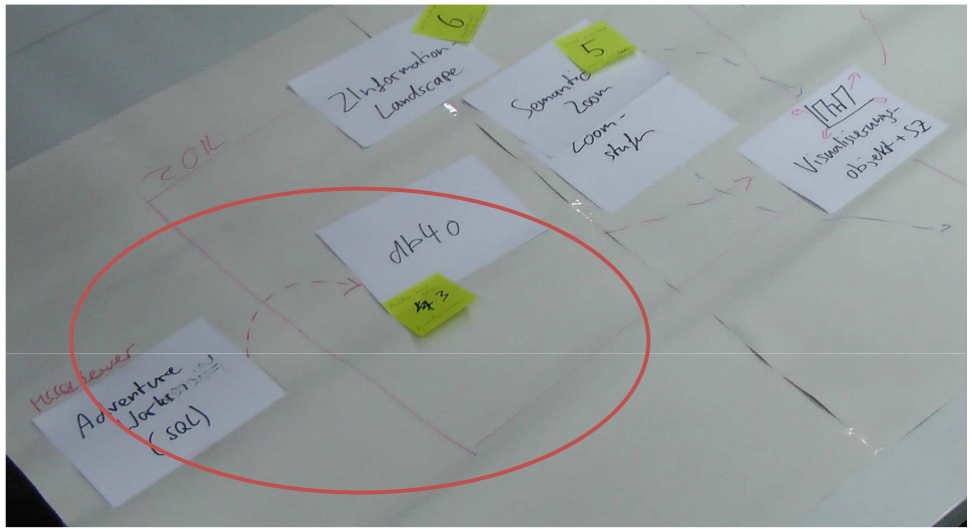
\includegraphics[scale=0.3]{figures/translation/translation_api_fig2.png}\\
    最初使用 db4o 作为存储后端的概念图
  \end{center}
\end{figure}

\begin{figure}
  \begin{center}
    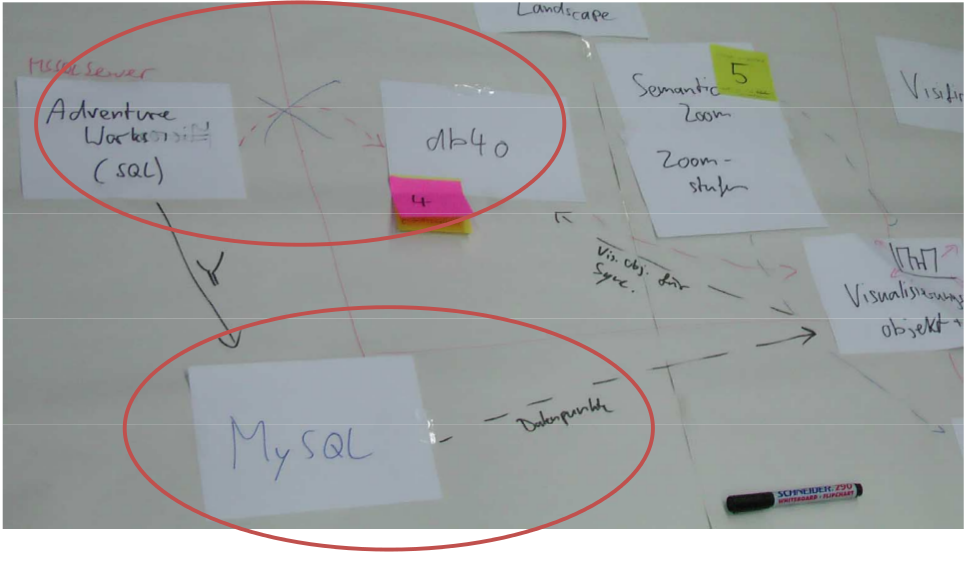
\includegraphics[scale=0.3]{figures/translation/translation_api_fig3.png}\\
    在概念图中加入 MySQL
  \end{center}
\end{figure}

\begin{figure}
  \begin{center}
    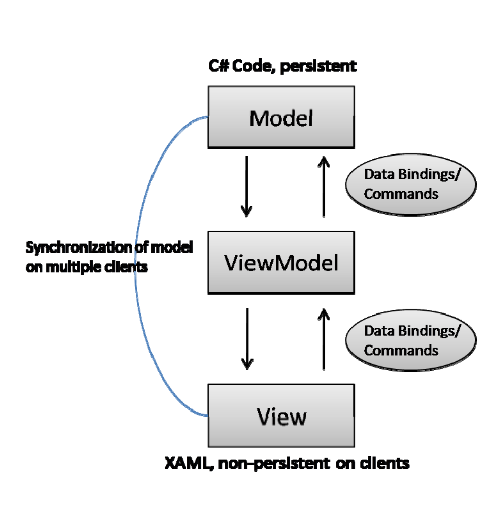
\includegraphics[scale=0.3]{figures/translation/translation_api_fig4.png}\\
    ZOIL 框架使用的 MVVM 设计
  \end{center}
\end{figure}

\begin{figure}
  \begin{center}
    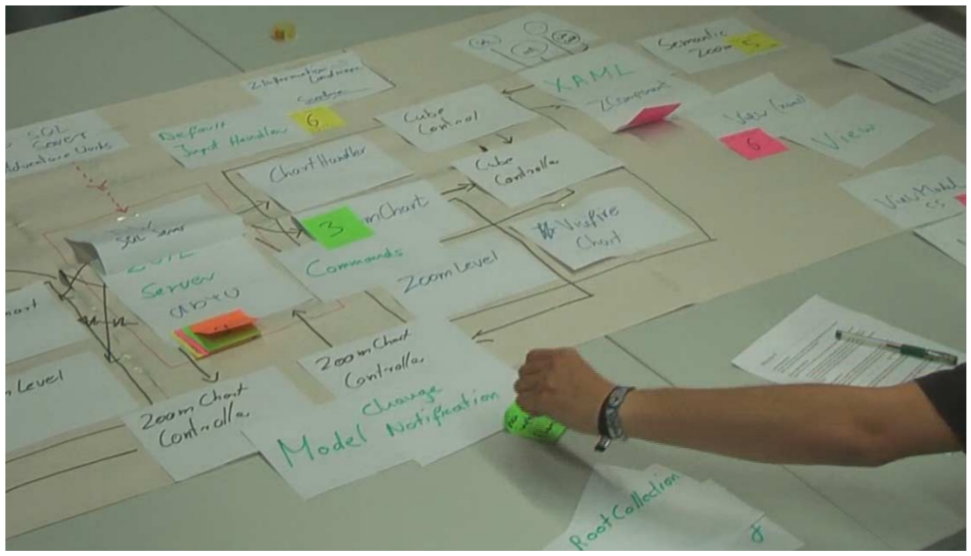
\includegraphics[scale=0.3]{figures/translation/translation_api_fig5.png}\\
    使用概念图模拟 MVVM 行为
  \end{center}
\end{figure}

\begin{figure}
  \begin{center}
    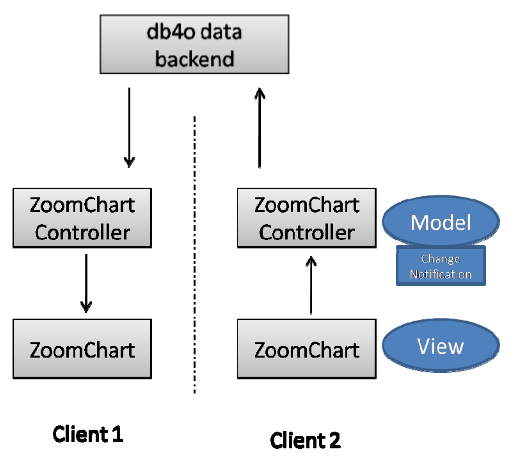
\includegraphics[scale=0.3]{figures/translation/translation_api_fig6.png}\\
    设计实现示意图
  \end{center}
\end{figure}

\textit{展望}
我们提出了一个纵向方法来评估一组API的可用性。这个方法包含可视概念图方法和问题日记方法,两个方法以跟踪纵向设计中的变化为关注点,来进行数据收集。我们的首次实验结果前景很好,我们将进一步精炼并扩展这个方法,并将其应用到更大更结构化的案例研究中,从而能描述出更多潜在好处的细节。一个有望的设计修改是减少用户在创建图的过程中的自由程度,使得能够出现在一些案例中更容易理解的结果的附加量化。我们还会比较我们的方法和传统的API可用性测试方法。

\newpage

\section*{外文译文原文}

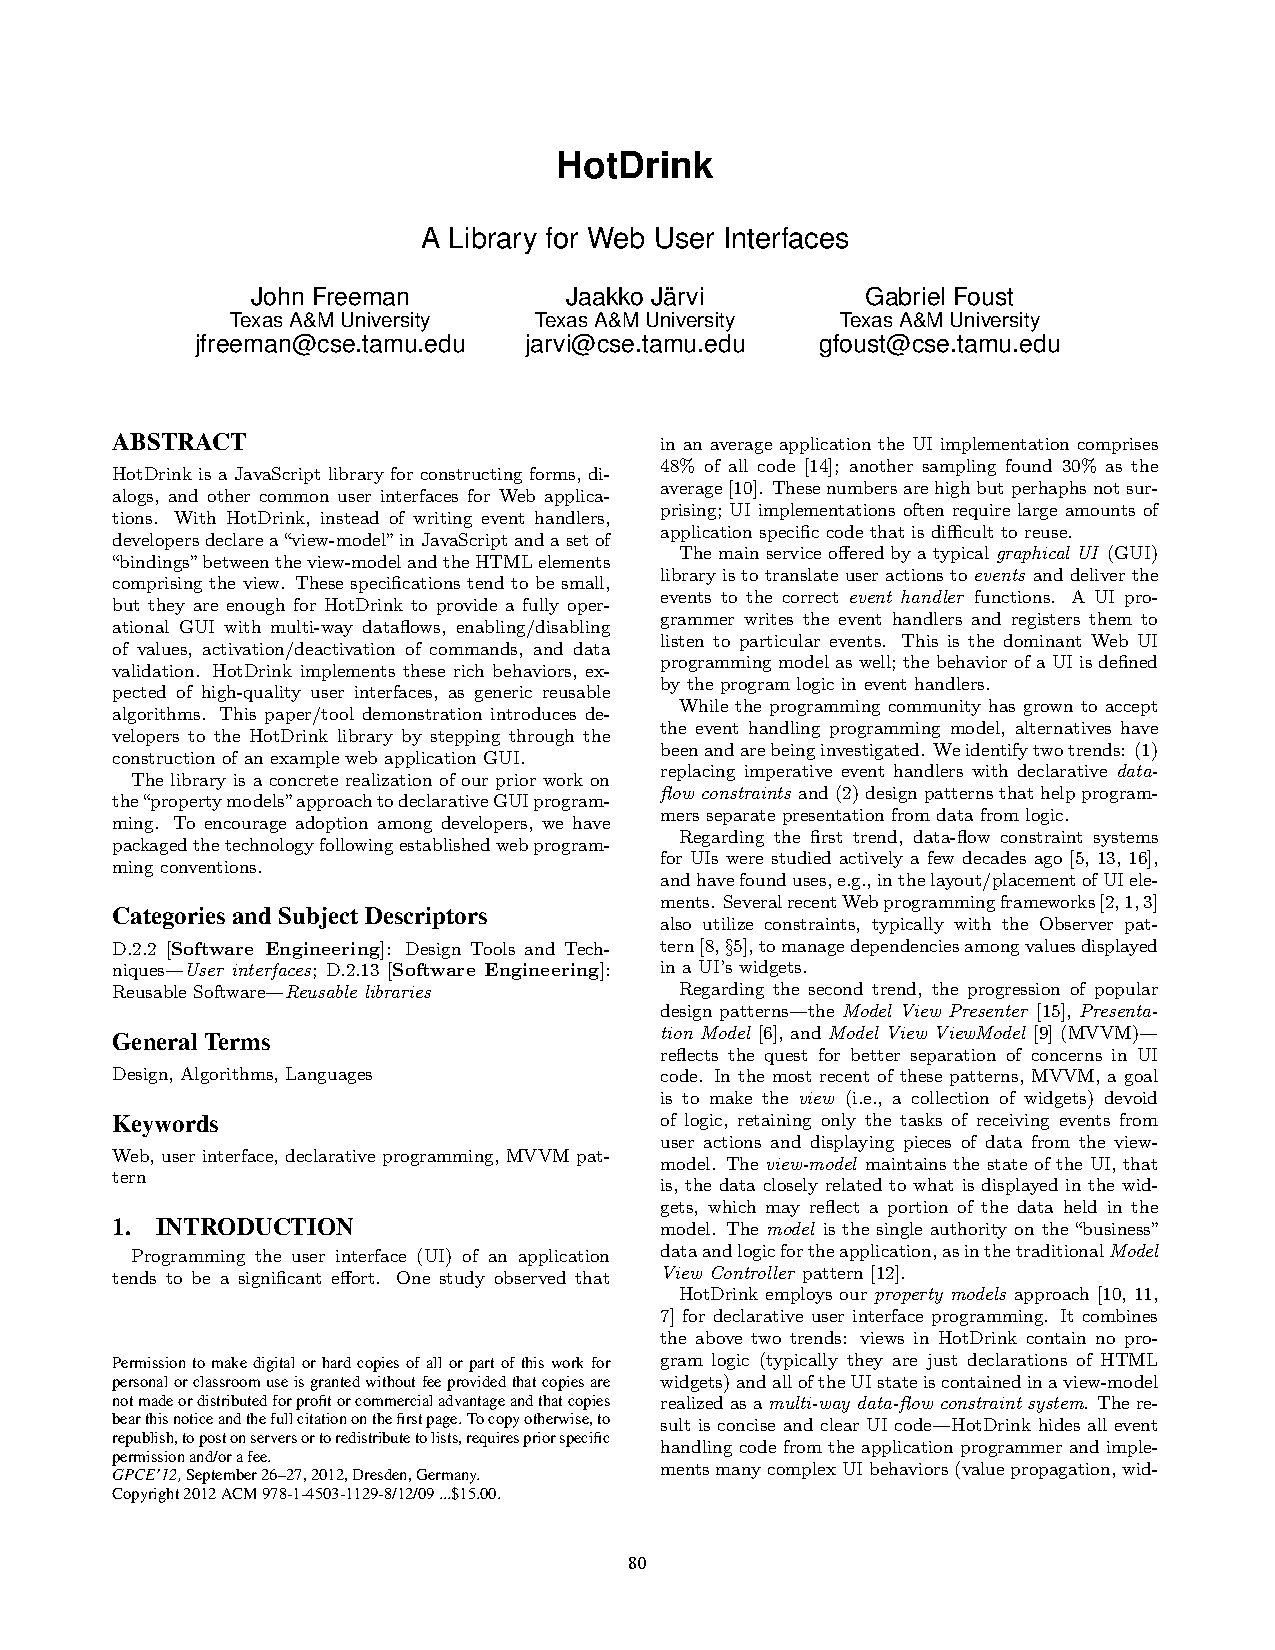
\includepdf[pages=-]{parts/translation/p80-freeman.pdf}

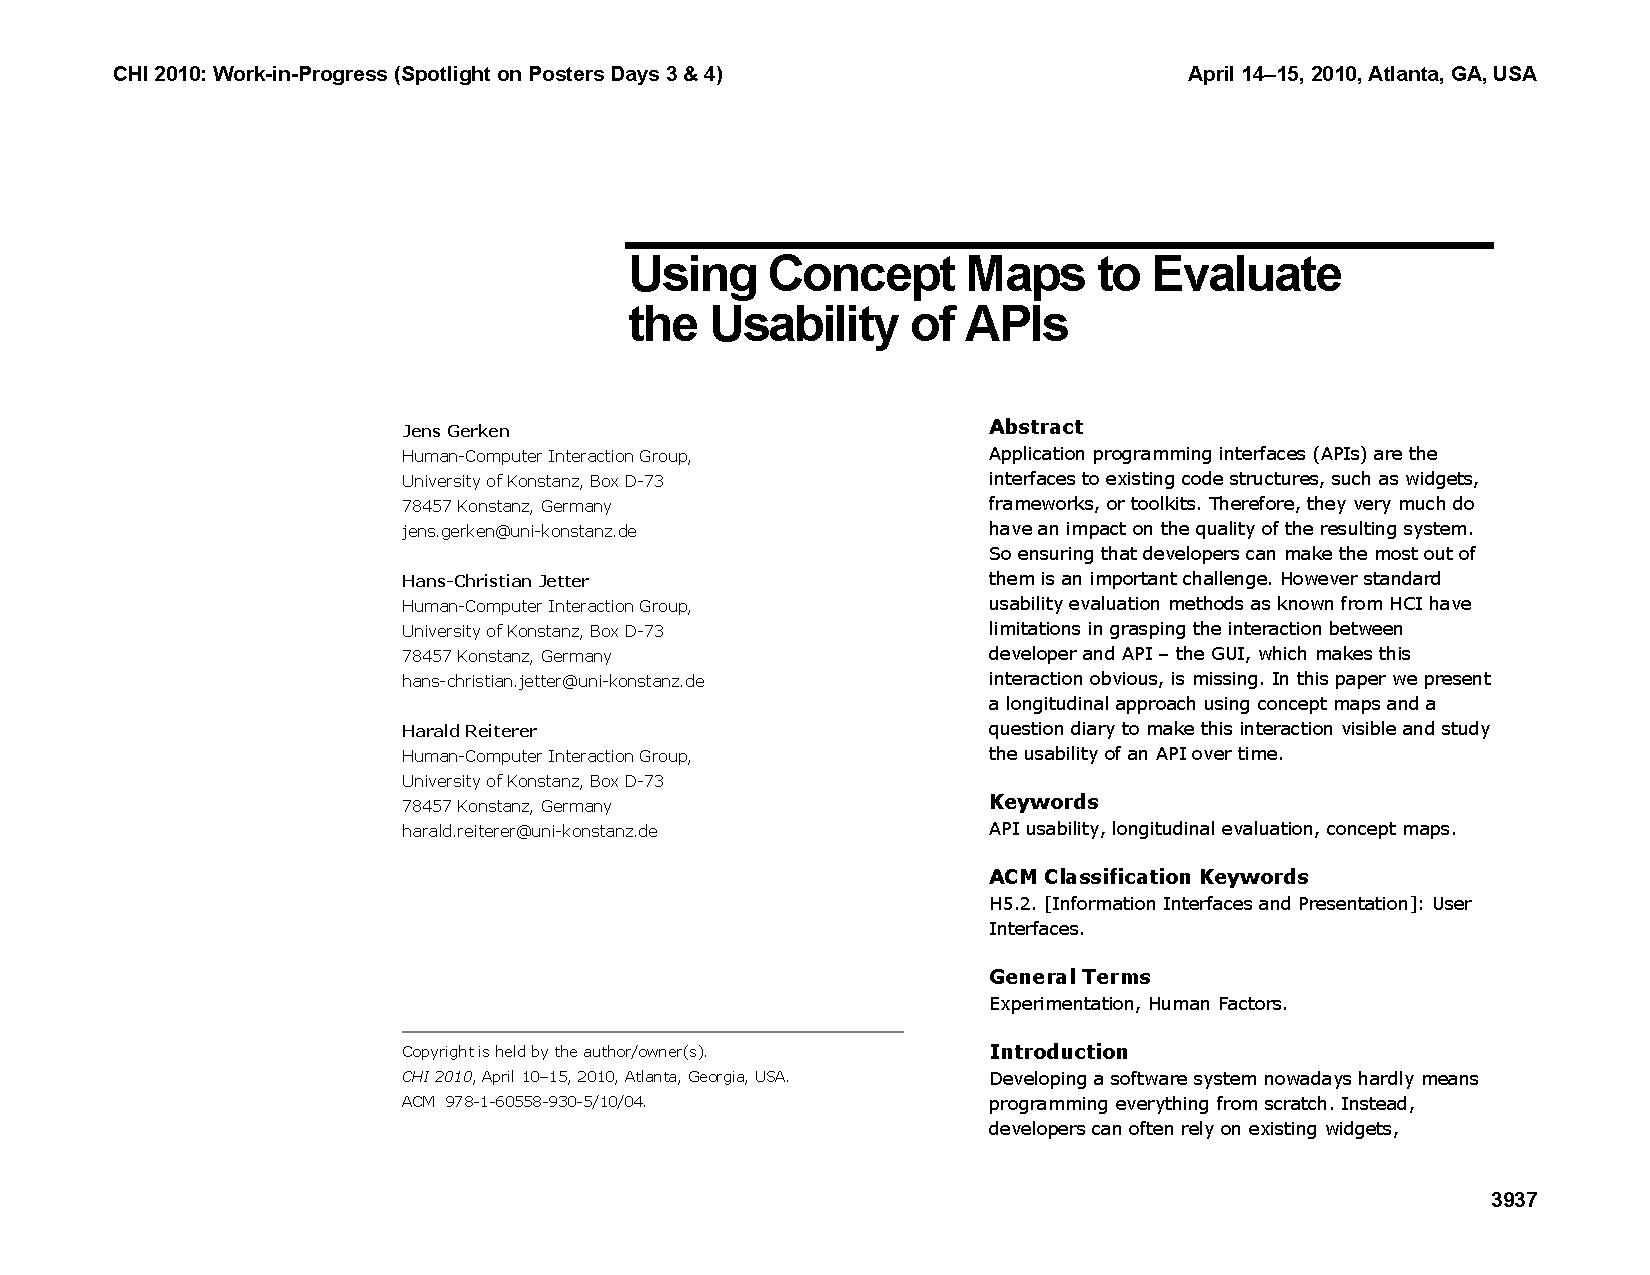
\includepdf[pages=-]{parts/translation/p3937-gerken.pdf}

